\documentclass[10p]{beamer}\usepackage[]{graphicx}\usepackage[]{color}
%% maxwidth is the original width if it is less than linewidth
%% otherwise use linewidth (to make sure the graphics do not exceed the margin)
\makeatletter
\def\maxwidth{ %
  \ifdim\Gin@nat@width>\linewidth
    \linewidth
  \else
    \Gin@nat@width
  \fi
}
\makeatother

\definecolor{fgcolor}{rgb}{0.345, 0.345, 0.345}
\newcommand{\hlnum}[1]{\textcolor[rgb]{0.686,0.059,0.569}{#1}}%
\newcommand{\hlstr}[1]{\textcolor[rgb]{0.192,0.494,0.8}{#1}}%
\newcommand{\hlcom}[1]{\textcolor[rgb]{0.678,0.584,0.686}{\textit{#1}}}%
\newcommand{\hlopt}[1]{\textcolor[rgb]{0,0,0}{#1}}%
\newcommand{\hlstd}[1]{\textcolor[rgb]{0.345,0.345,0.345}{#1}}%
\newcommand{\hlkwa}[1]{\textcolor[rgb]{0.161,0.373,0.58}{\textbf{#1}}}%
\newcommand{\hlkwb}[1]{\textcolor[rgb]{0.69,0.353,0.396}{#1}}%
\newcommand{\hlkwc}[1]{\textcolor[rgb]{0.333,0.667,0.333}{#1}}%
\newcommand{\hlkwd}[1]{\textcolor[rgb]{0.737,0.353,0.396}{\textbf{#1}}}%
\let\hlipl\hlkwb

\usepackage{framed}
\makeatletter
\newenvironment{kframe}{%
 \def\at@end@of@kframe{}%
 \ifinner\ifhmode%
  \def\at@end@of@kframe{\end{minipage}}%
  \begin{minipage}{\columnwidth}%
 \fi\fi%
 \def\FrameCommand##1{\hskip\@totalleftmargin \hskip-\fboxsep
 \colorbox{shadecolor}{##1}\hskip-\fboxsep
     % There is no \\@totalrightmargin, so:
     \hskip-\linewidth \hskip-\@totalleftmargin \hskip\columnwidth}%
 \MakeFramed {\advance\hsize-\width
   \@totalleftmargin\z@ \linewidth\hsize
   \@setminipage}}%
 {\par\unskip\endMakeFramed%
 \at@end@of@kframe}
\makeatother

\definecolor{shadecolor}{rgb}{.97, .97, .97}
\definecolor{messagecolor}{rgb}{0, 0, 0}
\definecolor{warningcolor}{rgb}{1, 0, 1}
\definecolor{errorcolor}{rgb}{1, 0, 0}
\newenvironment{knitrout}{}{} % an empty environment to be redefined in TeX

\usepackage{alltt}
\setbeamertemplate{footline}[page number]{}
\usepackage{lmodern}
\usepackage{graphicx}
\usepackage{fancybox}
\usepackage{graphics}
\usepackage{hyperref}
\usepackage{multirow}
\usepackage{etoolbox}
\usepackage{setspace}
\usepackage{booktabs}
\usepackage{array}
\usepackage{ragged2e}
\singlespacing

\mode<presentation>
{
%\usetheme{Frankfurt}
%\usecolortheme{seahorse}
%\setbeamercovered{transparent}
\usetheme{Singapore}
\usecolortheme{dolphin}
%\useoutertheme{infolines}
\useoutertheme[subsection=false]{smoothbars}
%\useoutertheme[footline=authortitle, subsection=false]{miniframes}
\useinnertheme{circles}
\usefonttheme{structurebold}

\setbeamercovered{transparent}
}

\newcommand{\blue}[1]{{\color{blue}{#1}}}
\newcommand{\red}[1]{{\color{red}{#1}}}
\newcommand{\gray}[1]{{\color{gray}{#1}}}

\setbeamercolor{subtitle}{fg=gray}

\makeatletter
\patchcmd{\beamer@sectionintoc}{\vskip1.5em}{\vskip0.5em}{}{}
\makeatother


%\author{Ryu, Hyuksu}
\author{Ryu, Hyuksu}
\institute{Naver Clova}
\title{A Tutorial for Linear Models and Linear Mixed Effects Models in R}
\subtitle{Experimental Phonetics} 
%\subtitle{실험음성학연구회} 
\date{\today}
\titlegraphic{
	
\includegraphics[height=.4cm]{../../Naver_logo.pdf}
	\hspace*{3cm}
	\includegraphics[height=.5cm]{../../Naver_clova_logo.pdf}
}

\AtBeginSection[]
{
\begin{frame}<beamer>
\frametitle{Outline}
\tableofcontents[currentsection,subsectionstyle=hide]
\end{frame}
}
\IfFileExists{upquote.sty}{\usepackage{upquote}}{}
\begin{document}


\begin{frame}
\maketitle
\end{frame}

\begin{frame}
\frametitle{T.O.C}
	\tableofcontents[subsectionstyle=hide]
\end{frame}

\section{Instruction}
\subsection{Instruction}

\begin{frame}
\frametitle{Before beginning}
Source of this tutorial
\begin{itemize}
  \item \href{http://www.bodowinter.com/tutorials.html}{Bodo Winter hompage} 
  \url{http://www.bodowinter.com/tutorials.html}
  \item \href{http://arxiv.org/pdf/1308.5499.pdf}{Linear models and linear mixed effects models in R}
  \url{http://arxiv.org/pdf/1308.5499.pdf}
\end{itemize}
\vspace{9pt}
Citation
\begin{itemize}
  \item Winter, B. (2013). Linear models and linear mixed effects models in R with linguistic applications. arXiv:1308.5499. 
\end{itemize}
\end{frame}

\begin{frame}
\frametitle{Instruction}
What we are dealing with?
\begin{enumerate}
\item Linear model
\item \alert{Linear mixed model} $\quad \leftarrow$
\end{enumerate}
\end{frame}

\section[Effects]{Fixed and random effects}
\subsection{Fixed and random effects}

\begin{frame}
\frametitle{Fixed and random effects}
In tutorial 1,
$$pitch \sim age + \epsilon$$
\begin{itemize}
\item age - fixed effect
	\begin{itemize}
	\item systematic part
	\end{itemize}

\item $\epsilon$ - random factor
	\begin{itemize}
	\item stochastic or probabilistic part
	\item to represent the deviations from our predictions
	\item ``random'' factors that we cannot control experimentally
	\end{itemize}
\item we will unpack this ``$\epsilon$''
\end{itemize}
\end{frame}

\begin{frame}
\frametitle{Model Description}
In this tutorial,
\begin{itemize}
\item interested in
	\begin{itemize}
	\item relationship b/w pitch and politeness
	\item relationship b/w pitch and sex
	\end{itemize}
\begin{displaymath}
pitch \sim politeness + sex + \epsilon
\end{displaymath}
\item politeness
	\begin{itemize}
	\item categorical factor with two levels - formal/informal
	\end{itemize}
\item \textbf{multiple} measures per subject
	\begin{itemize}
	\item violation of independence assumption
	\end{itemize}
\item Every person has different voice pitch
	\begin{itemize}
	\item rendering these different responses inter-dependent rather than independent.
	\end{itemize}
\end{itemize}
\end{frame}

\begin{frame}
\frametitle{Random effect}
Dealing with the situation, Add \textbf{random effect} for subject
\begin{itemize}
\item to resolve this non-independence 
	\begin{itemize}
	\item by assuming a different ``baseline'' pithc value for each subject
	\item for example, Subject 1 - 233 Hz (mean), and Subject 2 - 210 Hz



\centering
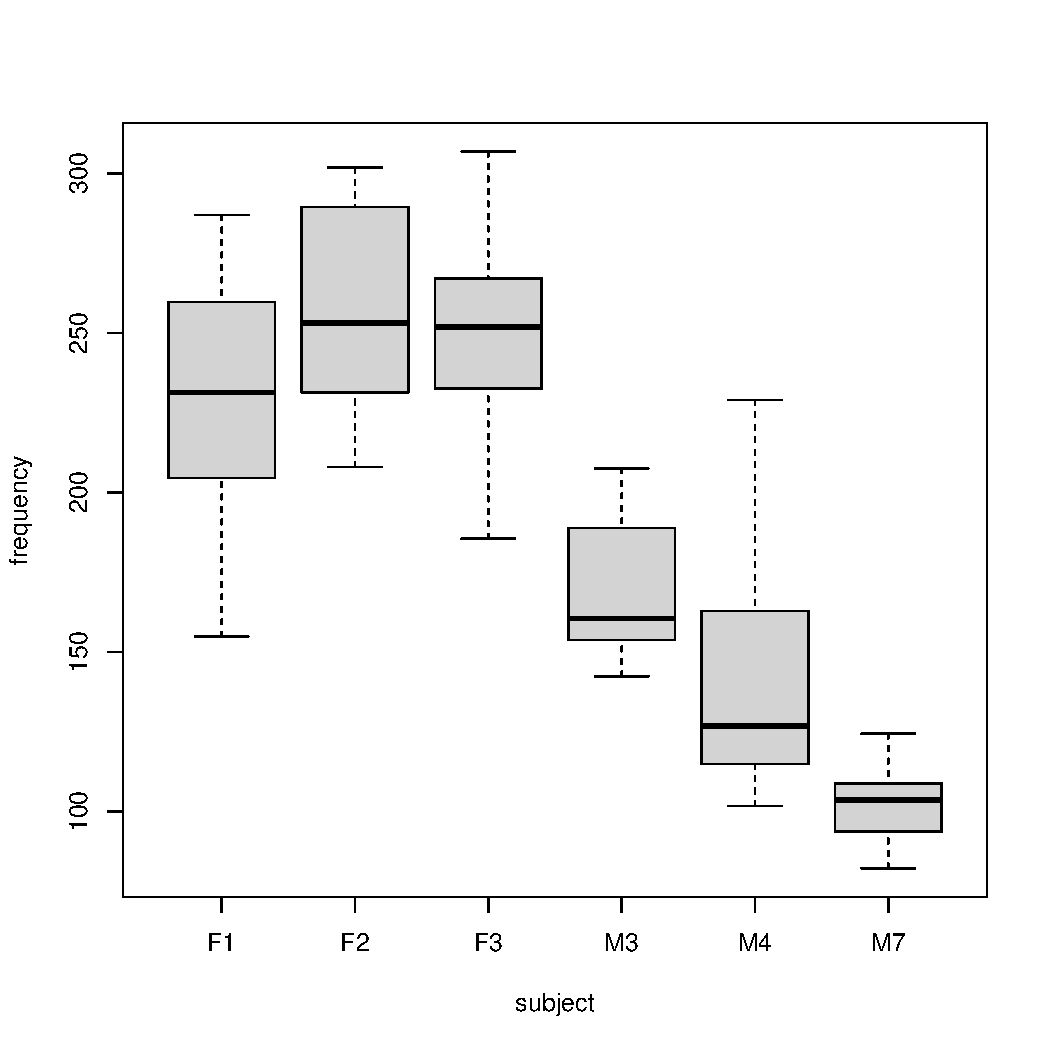
\includegraphics[scale=.3]{figure/box_subject-1}

	\end{itemize}
\end{itemize}
\end{frame}

\begin{frame}
\frametitle{Model description}
\begin{center}
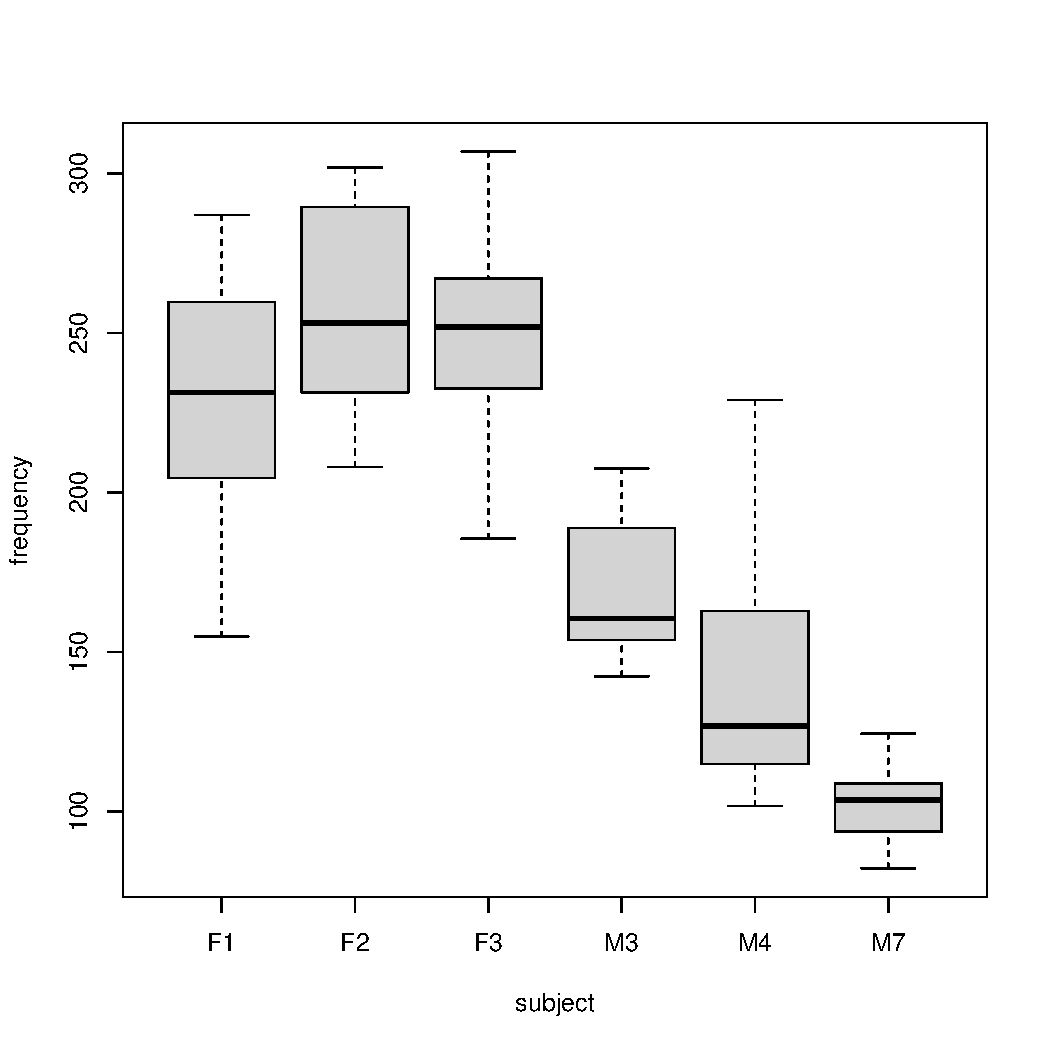
\includegraphics[scale=.25]{figure/box_subject-1}
\end{center}
From the box plot,
\begin{itemize}
\item pitch: male $<$ female
\item BUT, lots of individual variation
\end{itemize}

We can model these individual difference
\begin{itemize}
\item assuming different \textbf{random intercepts} for each subject
\end{itemize}
\end{frame}

\begin{frame}
\frametitle{Model description}
Why ``mixed'' model?
\begin{itemize}
\item{in addition to fixed effects,}
\item{we add one or more random effects}
  \begin{itemize}
  \item part of $\epsilon$ that we cannot control for
  \item in this case, a random effect for ``subject''
  \item this characterizes idiosyncratic variation that is due to individual differences
  \end{itemize}
\end{itemize}
Updated formula
\begin{displaymath}
pitch \sim politeness + sex + (1|subject) + \epsilon
\end{displaymath}
\end{frame}

\begin{frame}
\frametitle{Model description}
One more random thing
\begin{itemize}
\item item!
	\begin{itemize}
	\item 7 different scenarios (items)
	\item examples
		\begin{itemize}
		\item asking for a favor (polite/informal)
		\item excusing for coming too late (polite/informal)
		\end{itemize}
	\end{itemize}
\item also expect by-item variation
	\begin{itemize}
	\item For example,
	\item ``excusing for coming too late'' have overall higher pitch, regardless of the influence of politeness
	\item $\because$ it's more embarrassing than asking for a favor
	\item 
	\end{itemize}
\end{itemize}
\end{frame}

\begin{frame}
\frametitle{Model description}


\begin{center}
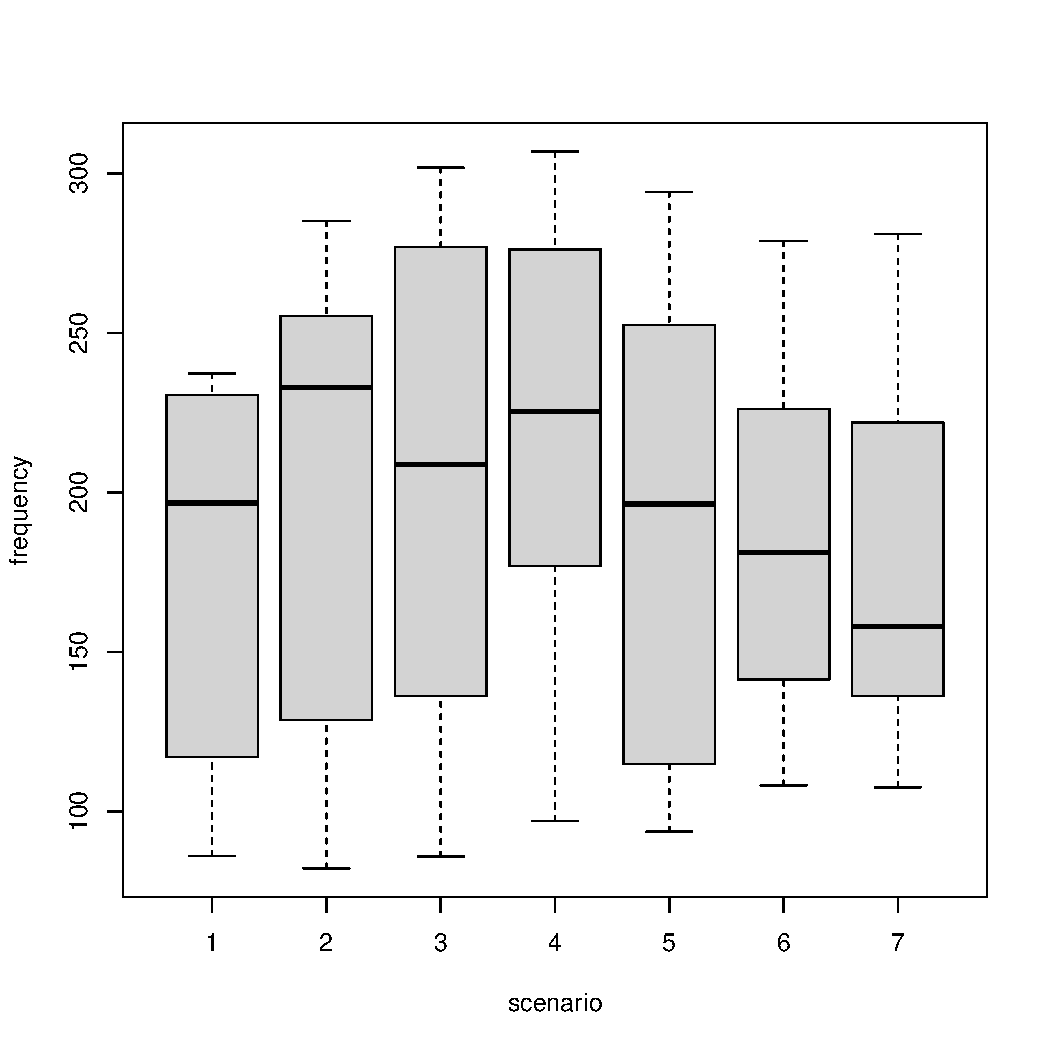
\includegraphics[scale=.22]{figure/box_item-1}
\end{center}
Variation b/w items
\begin{itemize}
\item not as big as the variation b/w subjects
\item but still noticeable, and better account for them in model
\end{itemize}

Adding an additional random effect
\begin{displaymath}
pitch \sim politeness + sex + (1|subject) + (1|item) + \epsilon
\end{displaymath}
\end{frame}

\begin{frame}
\frametitle{Mixed model}
The upshot is that
\begin{itemize}
\item mixed model give you much more flexibility than traditional model
\item take the full data into account
\item consider by-item variation and by-subject variation both in a single model
\end{itemize}
\end{frame}

\section[Mixed 1]{Mixed models 1}
\subsection{Mixed models in R}
\begin{frame}[fragile]{Pre-requisite}
For a start,
\begin{itemize}
\item need to install the R package \textit{lme4}
\begin{knitrout}
\definecolor{shadecolor}{rgb}{0.969, 0.969, 0.969}\color{fgcolor}\begin{kframe}
\begin{alltt}
\hlkwd{install.packages}\hlstd{(}\hlstr{"lme4"}\hlstd{)} \hlcom{# Linear Mixed Effect Model}
\end{alltt}
\end{kframe}
\end{knitrout}
\item after installation, laod the \textit{lme4} packages into R
\begin{knitrout}
\definecolor{shadecolor}{rgb}{0.969, 0.969, 0.969}\color{fgcolor}\begin{kframe}
\begin{alltt}
\hlkwd{library}\hlstd{(lme4)}
\end{alltt}
\end{kframe}
\end{knitrout}
\item a function we use for the mixed model
  \begin{itemize}
  \item \texttt{lmer()}
  \item the mixed model equivalent of the funtion \texttt{lm()} in linear model
  \end{itemize}

\end{itemize}
\end{frame}

\begin{frame}[fragile]
\frametitle{Loading data}
Loading data
\begin{knitrout}\scriptsize
\definecolor{shadecolor}{rgb}{0.969, 0.969, 0.969}\color{fgcolor}\begin{kframe}
\begin{alltt}
\hlstd{politeness}\hlkwb{=}\hlkwd{read.csv}\hlstd{(}\hlstr{"http://www.bodowinter.com/tutorial/politeness_data.csv"}\hlstd{)}
\end{alltt}
\end{kframe}
\end{knitrout}
\begin{knitrout}\scriptsize
\definecolor{shadecolor}{rgb}{0.969, 0.969, 0.969}\color{fgcolor}\begin{kframe}
\begin{alltt}
\hlkwd{summary}\hlstd{(politeness)}
\end{alltt}
\begin{verbatim}
##  subject gender    scenario attitude   frequency    
##  F1:14   F:42   Min.   :1   inf:42   Min.   : 82.2  
##  F2:14   M:42   1st Qu.:2   pol:42   1st Qu.:131.6  
##  F3:14          Median :4            Median :203.9  
##  M3:14          Mean   :4            Mean   :193.6  
##  M4:14          3rd Qu.:6            3rd Qu.:248.6  
##  M7:14          Max.   :7            Max.   :306.8  
##                                      NA's   :1
\end{verbatim}
\end{kframe}
\end{knitrout}
\begin{itemize}
\item \texttt{scenario} should be factor
\item should remove NA
\end{itemize}
\end{frame}

\begin{frame}[fragile]
\frametitle{Loading data}
\begin{itemize}
\item Factorize
\begin{knitrout}\scriptsize
\definecolor{shadecolor}{rgb}{0.969, 0.969, 0.969}\color{fgcolor}\begin{kframe}
\begin{alltt}
\hlstd{politeness}\hlopt{$}\hlstd{scenario} \hlkwb{=} \hlkwd{factor}\hlstd{(politeness}\hlopt{$}\hlstd{scenario)}
\end{alltt}
\end{kframe}
\end{knitrout}
\item Remove NA
\begin{knitrout}\scriptsize
\definecolor{shadecolor}{rgb}{0.969, 0.969, 0.969}\color{fgcolor}\begin{kframe}
\begin{alltt}
\hlstd{(idx} \hlkwb{=} \hlkwd{which}\hlstd{(}\hlkwd{is.na}\hlstd{(politeness}\hlopt{$}\hlstd{frequency)))}
\end{alltt}
\begin{verbatim}
## [1] 39
\end{verbatim}
\begin{alltt}
\hlstd{politeness} \hlkwb{=} \hlstd{politeness[}\hlopt{-}\hlstd{idx,]}
\end{alltt}
\end{kframe}
\end{knitrout}
\item Summary
\begin{knitrout}\scriptsize
\definecolor{shadecolor}{rgb}{0.969, 0.969, 0.969}\color{fgcolor}\begin{kframe}
\begin{alltt}
\hlkwd{summary}\hlstd{(politeness)}
\end{alltt}
\begin{verbatim}
##  subject gender scenario attitude   frequency    
##  F1:14   F:42   1:12     inf:42   Min.   : 82.2  
##  F2:14   M:41   2:12     pol:41   1st Qu.:131.6  
##  F3:14          3:12              Median :203.9  
##  M3:14          4:12              Mean   :193.6  
##  M4:13          5:12              3rd Qu.:248.6  
##  M7:14          6:11              Max.   :306.8  
##                 7:12
\end{verbatim}
\end{kframe}
\end{knitrout}

\end{itemize}
\end{frame}

\begin{frame}
\frametitle{Data structure}
Variables
\begin{itemize}
\item Dependent measure 
	\begin{itemize}
	\item Frequency - Hz
	\end{itemize}
\item Fixed
	\begin{itemize}
	\item Gender - M/F
	\item Attitude - inf/pol
	\end{itemize}
\item Random
	\begin{itemize}
	\item Subject
	\item Scenario
	\end{itemize}
\end{itemize}

\end{frame}

\begin{frame}[fragile]
\frametitle{Data structure}
Relationship b/w politeness \& pitch

\begin{center}
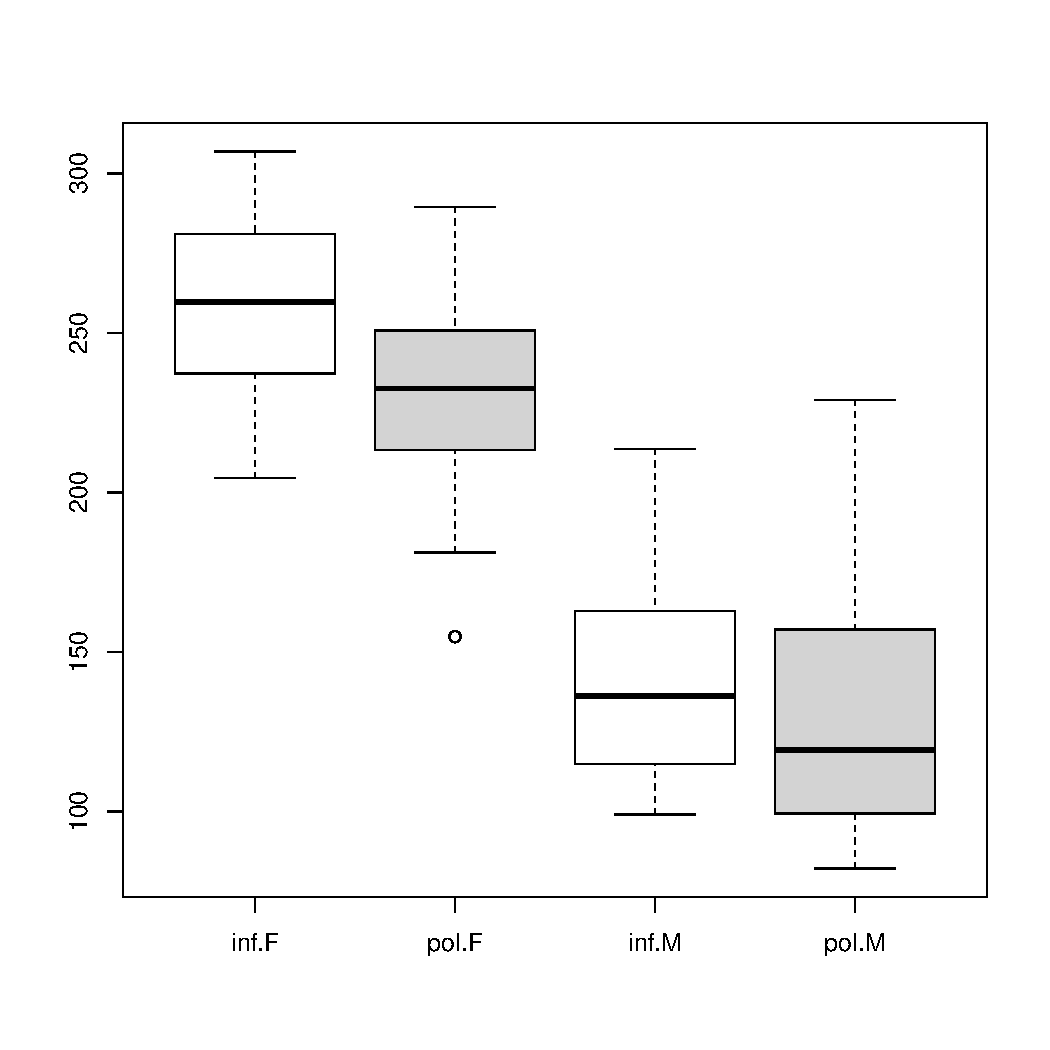
\includegraphics[scale=.28]{figure/box_freq-1}
\end{center}
\begin{itemize}
\item polite $<$ informal
\item But more overlap b/w two politeness categories for males than for females
\end{itemize}
\end{frame}

\begin{frame}[fragile]
\frametitle{Building mixed model}
How to build mixed model?
\begin{knitrout}\scriptsize
\definecolor{shadecolor}{rgb}{0.969, 0.969, 0.969}\color{fgcolor}\begin{kframe}
\begin{alltt}
\hlstd{politeness.model} \hlkwb{=} \hlkwd{lmer}\hlstd{(frequency} \hlopt{~} \hlstd{attitude} \hlopt{+} \hlstd{(}\hlnum{1}\hlopt{|}\hlstd{subject)} \hlopt{+}
        \hlstd{(}\hlnum{1}\hlopt{|}\hlstd{scenario),} \hlkwc{data}\hlstd{=politeness,} \hlkwc{REML}\hlstd{=}\hlnum{FALSE}\hlstd{)}
\end{alltt}
\end{kframe}
\end{knitrout}
Display the full result
\begin{knitrout}\scriptsize
\definecolor{shadecolor}{rgb}{0.969, 0.969, 0.969}\color{fgcolor}\begin{kframe}
\begin{alltt}
\hlkwd{summary}\hlstd{(politeness.model)}
\end{alltt}
\end{kframe}
\end{knitrout}
\end{frame}

\begin{frame}[fragile]
\frametitle{Building mixed model}
\begin{knitrout}\scriptsize
\definecolor{shadecolor}{rgb}{0.969, 0.969, 0.969}\color{fgcolor}\begin{kframe}
\begin{verbatim}
## Linear mixed model fit by maximum likelihood  ['lmerMod']
## Formula: frequency ~ attitude + (1 | subject) + (1 | scenario)
##    Data: politeness
## 
##      AIC      BIC   logLik deviance df.resid 
##    817.0    829.1   -403.5    807.0       78 
## 
## Scaled residuals: 
##     Min      1Q  Median      3Q     Max 
## -2.2127 -0.5906 -0.0598  0.5675  3.4584 
## 
## Random effects:
##  Groups   Name        Variance Std.Dev.
##  scenario (Intercept)  216.8   14.72   
##  subject  (Intercept) 3367.7   58.03   
##  Residual              637.0   25.24   
## Number of obs: 83, groups:  scenario, 7; subject, 6
## 
## Fixed effects:
##             Estimate Std. Error t value
## (Intercept)  202.588     24.646   8.220
## attitudepol  -19.692      5.546  -3.551
## 
## Correlation of Fixed Effects:
##             (Intr)
## attitudepol -0.111
\end{verbatim}
\end{kframe}
\end{knitrout}
\end{frame}

\begin{frame}[fragile]
\frametitle{Output}
General summary statistics
\begin{knitrout}\scriptsize
\definecolor{shadecolor}{rgb}{0.969, 0.969, 0.969}\color{fgcolor}\begin{kframe}
\begin{verbatim}
##       AIC       BIC    logLik  deviance  df.resid 
##  817.0395  829.1337 -403.5198  807.0395   78.0000
\end{verbatim}
\end{kframe}
\end{knitrout}
\begin{itemize}
\item Akaike's Information Criterion
\item log Likelihood
\item etc
\end{itemize}
\end{frame}

\begin{frame}
\frametitle{Output}

Random effects

\vspace{9pt}
\begin{tabular}{llll}

\toprule
Groups & Name & Variance & Std. Dev. \\
\midrule
scenario & (Intercept) & 219 & 14.80 \\
subject & (Intercept) & 4015 & 63.36 \\
Residual & & 646 & 25.42 \\
\bottomrule
\end{tabular}
\begin{itemize}
\item less variation in subject than scenario
\item which is expected by boxplot
\item ``Residual'' 
	\begin{itemize}
	\item stands for the variability that is not due to scenario or subject - our $\epsilon$
	\item ``random'' variation from the predicted that are not due to subjects and items
	\end{itemize}
\end{itemize}
\end{frame}

\begin{frame}[fragile]
\frametitle{Output}
Fixed effect
\begin{knitrout}\scriptsize
\definecolor{shadecolor}{rgb}{0.969, 0.969, 0.969}\color{fgcolor}\begin{kframe}
\begin{verbatim}
##              Estimate Std. Error   t value
## (Intercept) 202.58810  24.645978  8.219925
## attitudepol -19.69216   5.545759 -3.550851
\end{verbatim}
\end{kframe}
\end{knitrout}
\begin{itemize}
\item slope
	\begin{itemize}
\item same way of interpretation with linear model
\item informal $\rightarrow$ polite: -19.695Hz
	\end{itemize}
\item intercept 
	\begin{itemize}
	\item pitch at informal state
	\item fall halfway b/w males and females in the boxplot
	\item average of our data for the informal condition
	\item this is why we need gender as additional fixed effect
	\end{itemize}
\end{itemize}
\end{frame}

\section[Mixed 2]{Mixed models 2}
\subsection{building model}

\begin{frame}[fragile]
\frametitle{Building mixed model 2}
How to build mixed model?
\begin{knitrout}\scriptsize
\definecolor{shadecolor}{rgb}{0.969, 0.969, 0.969}\color{fgcolor}\begin{kframe}
\begin{alltt}
\hlstd{politeness.model.2} \hlkwb{=} \hlkwd{lmer}\hlstd{(frequency} \hlopt{~} \hlstd{attitude} \hlopt{+} \hlstd{gender} \hlopt{+} \hlstd{(}\hlnum{1}\hlopt{|}\hlstd{subject)} \hlopt{+} \hlstd{(}\hlnum{1}\hlopt{|}\hlstd{scenario),} \hlkwc{data}\hlstd{=politeness)}
\end{alltt}
\end{kframe}
\end{knitrout}

Display the full result
\begin{knitrout}\scriptsize
\definecolor{shadecolor}{rgb}{0.969, 0.969, 0.969}\color{fgcolor}\begin{kframe}
\begin{alltt}
\hlkwd{summary}\hlstd{(politeness.model.2)}
\end{alltt}
\end{kframe}
\end{knitrout}

\end{frame}

\begin{frame}[fragile]
\frametitle{Building mixed model 2}
\begin{knitrout}\scriptsize
\definecolor{shadecolor}{rgb}{0.969, 0.969, 0.969}\color{fgcolor}\begin{kframe}
\begin{verbatim}
## Linear mixed model fit by REML ['lmerMod']
## Formula: frequency ~ attitude + gender + (1 | subject) + (1 | scenario)
##    Data: politeness
## 
## REML criterion at convergence: 775.5
## 
## Scaled residuals: 
##     Min      1Q  Median      3Q     Max 
## -2.2591 -0.6236 -0.0772  0.5388  3.4795 
## 
## Random effects:
##  Groups   Name        Variance Std.Dev.
##  scenario (Intercept) 219.5    14.81   
##  subject  (Intercept) 615.6    24.81   
##  Residual             645.9    25.41   
## Number of obs: 83, groups:  scenario, 7; subject, 6
## 
## Fixed effects:
##             Estimate Std. Error t value
## (Intercept)  256.846     16.116  15.938
## attitudepol  -19.721      5.584  -3.532
## genderM     -108.516     21.013  -5.164
## 
## Correlation of Fixed Effects:
##             (Intr) atttdp
## attitudepol -0.173       
## genderM     -0.652  0.004
\end{verbatim}
\end{kframe}
\end{knitrout}
\end{frame}

\subsection{output}
\begin{frame}
\frametitle{Output}
Random effect

\vspace{9pt}
\begin{tabular}{llll}
\toprule
Groups & Name & Variance & Std.Dev. \\
\midrule
scenario & (Intercept) & 219.5 & 14.81 \\
subject & (Intercept) & 615.6 & 24.81 \\
Residual & & 645.9 & 25.42 \\
\bottomrule
\end{tabular}
\begin{itemize}
\item the variation of ``subject'' dropped drastically
\item By adding the effect of gender, we have shifted a considerable amount of the variance that was previously in the random effects component (difference b/w male and female individuals) to the fixed effects component
\end{itemize}
\end{frame}

\begin{frame}[fragile]
\frametitle{Output}
Fixed effects
\begin{knitrout}\scriptsize
\definecolor{shadecolor}{rgb}{0.969, 0.969, 0.969}\color{fgcolor}\begin{kframe}
\begin{verbatim}
##               Estimate Std. Error   t value
## (Intercept)  256.84627  16.115629 15.937712
## attitudepol  -19.72111   5.584028 -3.531699
## genderM     -108.51635  21.013326 -5.164168
\end{verbatim}
\end{kframe}
\end{knitrout}
\begin{itemize}
\item female $>$ male about 109 Hz
\item intercept is much higher
	\begin{itemize}
	\item represents the female category (for informal condition)
\item effect of attitude didn't change much
	\end{itemize}
\end{itemize}
\end{frame}

\section[Significance]{Statistical significance}
\subsection{p-value}
\begin{frame}
\frametitle{p-value}
p-value
\begin{itemize}
\item p-value for mixed models are not as straightforward as they are for the linear model
\item There are multiple approaches (still controversial)
\item \textbf{Likelihood Ratio Test} as a means to attain p-value
	\begin{itemize}
	\item the probability of seeing the data you collected given your model
	\item we compared a full model (with the fixed effects in question)
	\item against a reduced model without the effects in question
	\item by the result, we conclude that a fixed effect is significant if the difference b/w the likelihood of these two models is significant
	\end{itemize}
\end{itemize}
\end{frame}

\begin{frame}[fragile]
\frametitle{p-value}
Likelihood Ratio Test
\begin{itemize}
\item Note: should add the argument \alert{\texttt{REML=FALSE}}
\item construct null model
\begin{knitrout}\scriptsize
\definecolor{shadecolor}{rgb}{0.969, 0.969, 0.969}\color{fgcolor}\begin{kframe}
\begin{alltt}
\hlstd{politeness.null} \hlkwb{=} \hlkwd{lmer}\hlstd{(frequency} \hlopt{~} \hlstd{gender} \hlopt{+} \hlstd{(}\hlnum{1}\hlopt{|}\hlstd{subject)}
        \hlopt{+} \hlstd{(}\hlnum{1}\hlopt{|}\hlstd{scenario),} \hlkwc{data}\hlstd{=politeness,} \hlkwc{REML}\hlstd{=}\hlnum{FALSE}\hlstd{)}
\end{alltt}
\end{kframe}
\end{knitrout}
\item construct full model
\begin{knitrout}\scriptsize
\definecolor{shadecolor}{rgb}{0.969, 0.969, 0.969}\color{fgcolor}\begin{kframe}
\begin{alltt}
\hlstd{politeness.model} \hlkwb{=} \hlkwd{lmer}\hlstd{(frequency} \hlopt{~} \hlstd{attitude} \hlopt{+} \hlstd{gender}
        \hlopt{+} \hlstd{(}\hlnum{1}\hlopt{|}\hlstd{subject)} \hlopt{+} \hlstd{(}\hlnum{1}\hlopt{|}\hlstd{scenario),} \hlkwc{data}\hlstd{=politeness,} \hlkwc{REML}\hlstd{=}\hlnum{FALSE}\hlstd{)}
\end{alltt}
\end{kframe}
\end{knitrout}
\item perform the likelihood ratio test using the \texttt{anova()}
\begin{knitrout}\scriptsize
\definecolor{shadecolor}{rgb}{0.969, 0.969, 0.969}\color{fgcolor}\begin{kframe}
\begin{alltt}
\hlkwd{anova}\hlstd{(politeness.null, politeness.model)}
\end{alltt}
\end{kframe}
\end{knitrout}
full model:\quad frequency $\sim$ attitude + gender \\
reduced model:\quad frequency $\sim$ gender


\end{itemize}
\end{frame}

\begin{frame}[fragile]
\frametitle{p-value}
Result
\begin{knitrout}\scriptsize
\definecolor{shadecolor}{rgb}{0.969, 0.969, 0.969}\color{fgcolor}\begin{kframe}
\begin{verbatim}
## Data: politeness
## Models:
## politeness.null: frequency ~ gender + (1 | subject) + (1 | scenario)
## politeness.model: frequency ~ attitude + gender + (1 | subject) + (1 | scenario)
##                  Df    AIC    BIC  logLik deviance  Chisq Chi Df
## politeness.null   5 816.72 828.81 -403.36   806.72              
## politeness.model  6 807.10 821.61 -397.55   795.10 11.618      1
##                  Pr(>Chisq)    
## politeness.null                
## politeness.model  0.0006532 ***
## ---
## Signif. codes:  0 '***' 0.001 '**' 0.01 '*' 0.05 '.' 0.1 ' ' 1
\end{verbatim}
\end{kframe}
\end{knitrout}
Report
\begin{center}
\textrm{``... politeness affected pitch ($\chi^2$(1)=11.62, p=0.00065), lowering it by about 19.7 Hz $\pm$ 5.6 (standard errors)...''}
\end{center}
\end{frame}

\subsection{interaction}
\begin{frame}
\frametitle{interaction}
How to say regarding interaction
\begin{itemize}
\item If you have any an inter-dependence b/w two factors?
\item that is interaction
\item can test it the following way $\rightarrow$ likelihood test

full model:\quad frequency $\sim$ attitude + gender \\
reduced model:\quad frequency $\sim$ attitude * gender

\item compare the models using \texttt{anova()}
\item If \texttt{anova()} is significant, attitude and gender are significantly inter-dependent on each other

\end{itemize}
\end{frame}

\begin{frame}[fragile]
\frametitle{interaction}
\begin{knitrout}\scriptsize
\definecolor{shadecolor}{rgb}{0.969, 0.969, 0.969}\color{fgcolor}\begin{kframe}
\begin{alltt}
\hlstd{politeness.model} \hlkwb{=} \hlkwd{lmer}\hlstd{(frequency} \hlopt{~} \hlstd{attitude} \hlopt{+} \hlstd{gender} \hlopt{+} \hlstd{(}\hlnum{1}\hlopt{+}\hlstd{attitude}\hlopt{|}\hlstd{subject)}
        \hlopt{+} \hlstd{(}\hlnum{1}\hlopt{+}\hlstd{attitude}\hlopt{|}\hlstd{scenario),} \hlkwc{data}\hlstd{=politeness,} \hlkwc{REML}\hlstd{=}\hlnum{FALSE}\hlstd{)}
\hlstd{politeness.inter} \hlkwb{=} \hlkwd{lmer}\hlstd{(frequency} \hlopt{~} \hlstd{attitude} \hlopt{*} \hlstd{gender} \hlopt{+} \hlstd{(}\hlnum{1}\hlopt{+}\hlstd{attitude}\hlopt{|}\hlstd{subject)}
        \hlopt{+} \hlstd{(}\hlnum{1}\hlopt{+}\hlstd{attitude}\hlopt{|}\hlstd{scenario),} \hlkwc{data}\hlstd{=politeness,} \hlkwc{REML}\hlstd{=}\hlnum{FALSE}\hlstd{)}
\hlkwd{anova}\hlstd{(politeness.model, politeness.inter)}
\end{alltt}
\begin{verbatim}
## Data: politeness
## Models:
## politeness.model: frequency ~ attitude + gender + (1 + attitude | subject) + (1 + 
## politeness.model:     attitude | scenario)
## politeness.inter: frequency ~ attitude * gender + (1 + attitude | subject) + (1 + 
## politeness.inter:     attitude | scenario)
##                  Df    AIC    BIC  logLik deviance  Chisq Chi Df
## politeness.model 10 814.90 839.09 -397.45   794.90              
## politeness.inter 11 814.89 841.50 -396.45   792.89 2.0023      1
##                  Pr(>Chisq)
## politeness.model           
## politeness.inter     0.1571
\end{verbatim}
\end{kframe}
\end{knitrout}
No significant interaction here
\end{frame}

\section[Random slope]{Random slope and random intercepts}
\subsection{slope}

\begin{frame}[fragile]
\frametitle{random slopes vs. random intercepts}
the coefficients of the model by subject and by item
\begin{knitrout}\footnotesize
\definecolor{shadecolor}{rgb}{0.969, 0.969, 0.969}\color{fgcolor}\begin{kframe}
\begin{alltt}
\hlkwd{coef}\hlstd{(politeness.model)}
\end{alltt}
\end{kframe}
\end{knitrout}
\end{frame}

\begin{frame}[fragile]
\frametitle{random slopes vs. random intercepts}
\begin{knitrout}\scriptsize
\definecolor{shadecolor}{rgb}{0.969, 0.969, 0.969}\color{fgcolor}\begin{kframe}
\begin{verbatim}
## $scenario
##   (Intercept) attitudepol   genderM
## 1    245.2603   -20.43832 -110.8021
## 2    263.3012   -15.94385 -110.8021
## 3    269.1432   -20.63361 -110.8021
## 4    276.8309   -16.30132 -110.8021
## 5    256.0579   -19.40575 -110.8021
## 6    246.8605   -21.94816 -110.8021
## 7    248.4702   -23.55752 -110.8021
## 
## $subject
##    (Intercept) attitudepol   genderM
## F1    243.8053   -20.68245 -110.8021
## F2    266.7321   -19.17028 -110.8021
## F3    260.1484   -19.60452 -110.8021
## M3    285.6958   -17.91950 -110.8021
## M4    264.1982   -19.33741 -110.8021
## M7    227.3551   -21.76744 -110.8021
## 
## attr(,"class")
## [1] "coef.mer"
\end{verbatim}
\end{kframe}
\end{knitrout}
\end{frame}

\begin{frame}
\frametitle{random slopes vs. random intercepts}
Result
\begin{itemize}
\item each scenario and subject is assigned \textbf{a different intercept}
  \begin{itemize}
  \item by-subject and by-item variability
  \end{itemize}
\item the fixed effects (attitude and gender) are \textbf{all the same} for all subjects and items
\item \textbf{random intercept model}
  \begin{itemize}
  \item baseline-differences in pitch
  \item but, effect of politeness and gender is the same for all subjects and items
  \end{itemize}
\item is it a valid assumption?
  \begin{itemize}
  \item the effect of politeness might be different for differnt items and subjects
  \end{itemize}
\item so, we need a \textbf{random slope model}
\end{itemize}
\end{frame}

\subsection{Random slope model}
\begin{frame}[fragile]
\frametitle{Random slope model}
What we changed
\begin{itemize}
\item only the random effects
\item \texttt{(1+attitude|subject)}
  \begin{itemize}
  \item this notation means differing responses to attitude
  \item as well as differing baseline-levels of frequency (intercept)
  \end{itemize}
\end{itemize}
Model
\begin{knitrout}\scriptsize
\definecolor{shadecolor}{rgb}{0.969, 0.969, 0.969}\color{fgcolor}\begin{kframe}
\begin{alltt}
\hlstd{politeness.model} \hlkwb{=} \hlkwd{lmer}\hlstd{(frequency} \hlopt{~} \hlstd{attitude} \hlopt{+} \hlstd{gender}
                        \hlopt{+} \hlstd{(}\hlnum{1}\hlopt{+}\hlstd{attitude}\hlopt{|}\hlstd{subject)} \hlopt{+} \hlstd{(}\hlnum{1}\hlopt{+}\hlstd{attitude}\hlopt{|}\hlstd{scenario),}
                        \hlkwc{data}\hlstd{=politeness,} \hlkwc{REML}\hlstd{=}\hlnum{FALSE}\hlstd{)}
\end{alltt}
\end{kframe}
\end{knitrout}
Coefficients of this updated model
\begin{knitrout}\footnotesize
\definecolor{shadecolor}{rgb}{0.969, 0.969, 0.969}\color{fgcolor}\begin{kframe}
\begin{alltt}
\hlkwd{coef}\hlstd{(politeness.model)}
\end{alltt}
\end{kframe}
\end{knitrout}
\end{frame}

\begin{frame}[fragile]
\frametitle{Random slope model}
\begin{knitrout}\scriptsize
\definecolor{shadecolor}{rgb}{0.969, 0.969, 0.969}\color{fgcolor}\begin{kframe}
\begin{verbatim}
## $scenario
##   (Intercept) attitudepol   genderM
## 1    245.2603   -20.43832 -110.8021
## 2    263.3012   -15.94385 -110.8021
## 3    269.1432   -20.63361 -110.8021
## 4    276.8309   -16.30132 -110.8021
## 5    256.0579   -19.40575 -110.8021
## 6    246.8605   -21.94816 -110.8021
## 7    248.4702   -23.55752 -110.8021
## 
## $subject
##    (Intercept) attitudepol   genderM
## F1    243.8053   -20.68245 -110.8021
## F2    266.7321   -19.17028 -110.8021
## F3    260.1484   -19.60452 -110.8021
## M3    285.6958   -17.91950 -110.8021
## M4    264.1982   -19.33741 -110.8021
## M7    227.3551   -21.76744 -110.8021
## 
## attr(,"class")
## [1] "coef.mer"
\end{verbatim}
\end{kframe}
\end{knitrout}
\end{frame}

\begin{frame}
\frametitle{Random slope model}
Interpretation
\begin{itemize}
\item the column for politeness is different for each subject and item
\item but it is always negative and quite similar to each other
\item means that despite individual variation, there is also consistency in how politeness affects the voice
  \begin{itemize}
  \item for all of speakers, the voice tends to go down in polite speech,
  \item but for some people it goes down slightly more so than for others
  \end{itemize}
\item coefficients of gender do not change, since we did not specify random slope for the factor
\end{itemize}
\end{frame}

\begin{frame}[fragile]
\frametitle{Random slope model}
Obtain p-value in random slope model
\begin{itemize}
\item Likelihood ratio test
\item Comparison of full model and the reduced model
\begin{knitrout}\scriptsize
\definecolor{shadecolor}{rgb}{0.969, 0.969, 0.969}\color{fgcolor}\begin{kframe}
\begin{alltt}
\hlstd{politeness.model} \hlkwb{=} \hlkwd{lmer}\hlstd{(frequency} \hlopt{~} \hlstd{attitude} \hlopt{+} \hlstd{gender}
                        \hlopt{+} \hlstd{(}\hlnum{1}\hlopt{+}\hlstd{attitude}\hlopt{|}\hlstd{subject)}\hlopt{+}\hlstd{(}\hlnum{1}\hlopt{+}\hlstd{attitude}\hlopt{|}\hlstd{scenario),}
                        \hlkwc{data}\hlstd{=politeness,} \hlkwc{REML}\hlstd{=}\hlnum{FALSE}\hlstd{)}
\hlstd{politeness.null} \hlkwb{=} \hlkwd{lmer}\hlstd{(frequency} \hlopt{~} \hlstd{gender}
                       \hlopt{+} \hlstd{(}\hlnum{1}\hlopt{+}\hlstd{attitude}\hlopt{|}\hlstd{subject)} \hlopt{+} \hlstd{(}\hlnum{1}\hlopt{+}\hlstd{attitude}\hlopt{|}\hlstd{scenario),}
                       \hlkwc{data}\hlstd{=politeness,} \hlkwc{REML} \hlstd{=} \hlnum{FALSE}\hlstd{)}
\end{alltt}
\end{kframe}
\end{knitrout}
\item need the same random effects structure (random slope model)
\end{itemize}
\end{frame}

\begin{frame}[fragile]
\frametitle{Random slope model}
Likelyhood ratio test
\begin{knitrout}\scriptsize
\definecolor{shadecolor}{rgb}{0.969, 0.969, 0.969}\color{fgcolor}\begin{kframe}
\begin{alltt}
\hlkwd{anova}\hlstd{(politeness.null, politeness.model)}
\end{alltt}
\begin{verbatim}
## Data: politeness
## Models:
## politeness.null: frequency ~ gender + (1 + attitude | subject) + (1 + attitude | 
## politeness.null:     scenario)
## politeness.model: frequency ~ attitude + gender + (1 + attitude | subject) + (1 + 
## politeness.model:     attitude | scenario)
##                  Df    AIC    BIC  logLik deviance  Chisq Chi Df
## politeness.null   9 819.61 841.37 -400.80   801.61              
## politeness.model 10 814.90 839.09 -397.45   794.90 6.7082      1
##                  Pr(>Chisq)   
## politeness.null               
## politeness.model   0.009597 **
## ---
## Signif. codes:  0 '***' 0.001 '**' 0.01 '*' 0.05 '.' 0.1 ' ' 1
\end{verbatim}
\end{kframe}
\end{knitrout}
Siginificant result!
\end{frame}

\begin{frame}
\frametitle{Why random slope?}
Questions?
\begin{itemize}
\item Which random slopes should I specify?
\item Are random slopes necessry at all?
\end{itemize}

Answer!
\begin{itemize}
\item it makes lots of sense to include random slopes most of the time
\item it is reasonable to expect that the effect of an experimental manipulation is not going to be the same for all items.
\item several researches  have shown that mixed models w/o random slopes have a relatively high Type I error rate
  \begin{itemize}
  \item They tend to find a lot of significant results which are actually due to chance
  \end{itemize}
\end{itemize}
\end{frame}

\begin{frame}
\frametitle{Why random slope?}
In this model, why did we have random slope for only attitude, not gender? 
\begin{itemize}
\item we were not interested in gender differences
\item they are well worth controlling for
\item therefore, we only modeled by-subject and by-item variability in how politeness affects pitch
\end{itemize}
\end{frame}

\section[Assume]{Assumptions}
\subsection{Assumptions}
\begin{frame}
\frametitle{Assumptions in LM}
Assumptions in LM
\begin{enumerate}
\item Linearity
\item Absense of collinearity
\item Homoskedasticity
\item Normality of residuals
\item Absense of influential data points
\item Independence
\end{enumerate}

Good news!
\begin{itemize}
\item Everything applies straightforwardly to mixed model
\end{itemize}

\end{frame}

\begin{frame}
\frametitle{Independence}
Why did we move to mixed model?
\begin{itemize}
\item to resolve non-independencies in our data
\end{itemize}

Cautions
\begin{itemize}
\item still should be cautious in violation
\item missing fixed or random effects cause independence violation
\item Choose fixed and random effects carefully 
\end{itemize}
\end{frame}

\begin{frame}[fragile]
\frametitle{Influential data points}
Infuential data points in LM
\begin{itemize}
\item \texttt{dfbeta()} function
\end{itemize}

But, in the mixed model,
\begin{itemize}
\item \texttt{dfbeta()} function does not work
\item ``leave-one-out'' diagnosis by hand
\item example script for leave-one-out diagnosis for attitude
\begin{knitrout}\scriptsize
\definecolor{shadecolor}{rgb}{0.969, 0.969, 0.969}\color{fgcolor}\begin{kframe}
\begin{alltt}
\hlstd{all.res.attitude} \hlkwb{=} \hlkwd{numeric}\hlstd{(}\hlkwd{nrow}\hlstd{(politeness))}
\hlstd{all.res.gender} \hlkwb{=} \hlkwd{numeric}\hlstd{(}\hlkwd{nrow}\hlstd{(politeness))}

\hlkwa{for}\hlstd{(i} \hlkwa{in} \hlnum{1}\hlopt{:}\hlkwd{nrow}\hlstd{(politeness))\{}
  \hlstd{myfullmodel} \hlkwb{=} \hlkwd{lmer}\hlstd{(frequency} \hlopt{~} \hlstd{attitude} \hlopt{+} \hlstd{gender} \hlopt{+}
                       \hlstd{(}\hlnum{1}\hlopt{+}\hlstd{attitude}\hlopt{|}\hlstd{subject)}\hlopt{+}\hlstd{(}\hlnum{1}\hlopt{+}\hlstd{attitude}\hlopt{|}\hlstd{scenario),}
                   \hlkwc{data}\hlstd{=politeness[}\hlopt{-}\hlstd{i,],} \hlkwc{REML}\hlstd{=}\hlnum{FALSE}\hlstd{)}
  \hlcom{# 1- intercept, 2-attitude, 3-gender }
  \hlstd{all.res.attitude[i]} \hlkwb{=} \hlkwd{fixef}\hlstd{(myfullmodel)[}\hlnum{2}\hlstd{]}
  \hlstd{all.res.gender[i]} \hlkwb{=} \hlkwd{fixef}\hlstd{(myfullmodel)[}\hlnum{3}\hlstd{]} \hlcom{# }
\hlstd{\}}
\end{alltt}
\end{kframe}
\end{knitrout}
\end{itemize}
\end{frame}

\section[Final]{Final notes on random vs. fixed}
\subsection{Final}
\begin{frame}
\frametitle{Final notes}
More about fixed and random effects
\begin{itemize}
\item random effect
  \begin{itemize}
  \item Generally something that can be expected to have 
  \item a non-systematic, idiosyncratic, unpredictable, or ``random'' influence on data
  \item often ``subject'' and ``item''
  \item the things you generally want to generalize over the idiosyncrasies of individual subjects and items
  \item generally ``sample'' from the population of interests
  \item far away from ``exhausting the population'' b/c many many more subjects or items that you could have tested
  \end{itemize}
  
\item fixed effect
  \begin{itemize}
  \item are expected to have a systematic and predictable influence on your data
  \item ``exhaust the population of interest''
  \item ``exhaust the levels of a factor''
  \item For example, gender has only two levels and, by two categories, exhausts the category gender
  \end{itemize}
\end{itemize}
\end{frame}

\subsection{Write-up}
\begin{frame}[fragile]
\frametitle{Write-up}
More things to consider
\begin{enumerate}
\item Reproducibility
\item Coefficients
\item Citation
\end{enumerate}
\end{frame}

\begin{frame}
\frametitle{Write-up}
Reproducibility
\begin{itemize}
\item need to describe the model to such an extent that people can reproduce the analysis
\item ask yourself the question
\item ``Would I be able to recreate the analysis given the information that I provided?''
\item If the answer is ``yes'', write-up is good
\end{itemize}

Coefficients
\begin{itemize}
\item report the actual coefficients/estimates
\item not just whether an effect is significant or not
\item also mention standard errors
\end{itemize}
\end{frame}

\begin{frame}[fragile]
\frametitle{Write-up}
Citation for R: citation()
\begin{knitrout}\scriptsize
\definecolor{shadecolor}{rgb}{0.969, 0.969, 0.969}\color{fgcolor}\begin{kframe}
\begin{verbatim}
## 
## To cite R in publications use:
## 
##   R Core Team (2017). R: A language and environment for
##   statistical computing. R Foundation for Statistical Computing,
##   Vienna, Austria. URL https://www.R-project.org/.
## 
## A BibTeX entry for LaTeX users is
## 
##   @Manual{,
##     title = {R: A Language and Environment for Statistical Computing},
##     author = {{R Core Team}},
##     organization = {R Foundation for Statistical Computing},
##     address = {Vienna, Austria},
##     year = {2017},
##     url = {https://www.R-project.org/},
##   }
## 
## We have invested a lot of time and effort in creating R, please
## cite it when using it for data analysis. See also
## 'citation("pkgname")' for citing R packages.
\end{verbatim}
\end{kframe}
\end{knitrout}
\end{frame}

\begin{frame}[fragile]
\frametitle{Write-up}
Citation for package `lme4'
\begin{knitrout}\scriptsize
\definecolor{shadecolor}{rgb}{0.969, 0.969, 0.969}\color{fgcolor}\begin{kframe}
\begin{alltt}
\hlkwd{citation}\hlstd{(}\hlstr{'lme4'}\hlstd{)}
\end{alltt}
\begin{verbatim}
## 
## To cite lme4 in publications use:
## 
##   Douglas Bates, Martin Maechler, Ben Bolker, Steve Walker (2015).
##   Fitting Linear Mixed-Effects Models Using lme4. Journal of
##   Statistical Software, 67(1), 1-48. doi:10.18637/jss.v067.i01.
## 
## A BibTeX entry for LaTeX users is
## 
##   @Article{,
##     title = {Fitting Linear Mixed-Effects Models Using {lme4}},
##     author = {Douglas Bates and Martin M{\"a}chler and Ben Bolker and Steve Walker},
##     journal = {Journal of Statistical Software},
##     year = {2015},
##     volume = {67},
##     number = {1},
##     pages = {1--48},
##     doi = {10.18637/jss.v067.i01},
##   }
\end{verbatim}
\end{kframe}
\end{knitrout}
\end{frame}

\begin{frame}
\frametitle{Example Writing}
\begin{block}{Example}
\rmfamily \small \justifying
We used R (R Core Team, 2014) and \textit{lme4} (Bates, Maechler, Bolker \& Walker, 2014) to perform a linear mixed effects analysis of the relationship between pitch and politeness. 
As fixed effects, we entered politeness and gender (without interaction term) into the model. As random effects, we had intercepts for subjects and items, as well as by-subject and by-item random slopes for the effect of politeness. 
Visual inspection of residual plots did not reveal any obvious deviations from homoscedasticity or normality. 
P-values were obtained by likelihood ratio tests of the full model with the effect in question against the model without the effect in question.
\end{block}
\end{frame}

\end{document}
